%!TEX root = ../Main.tex

% 第一章
\chapter{绪论}
\section{研究背景及意义}
期刊引用\cite{journalkey}没有夹带私货w。

会议引用\cite{conferencekey}没办法夹带私货w。

\section{国内外研究现状}
\subsection{相关研究方向一}

描述一下呗

\subsubsection{方法类别一}
xxx

\subsubsection{方法类别二}

记得总结下

\subsection{相关研究方向二}

记得总结下

\section{研究内容与创新点}
\subsection{研究内容}
图\ref{fig:research framework}展示了本文的主要研究框架。

\begin{figure}[h!] % 解决浮动体太多空白的问题 https://zhuanlan.zhihu.com/p/648268901
	\centering
	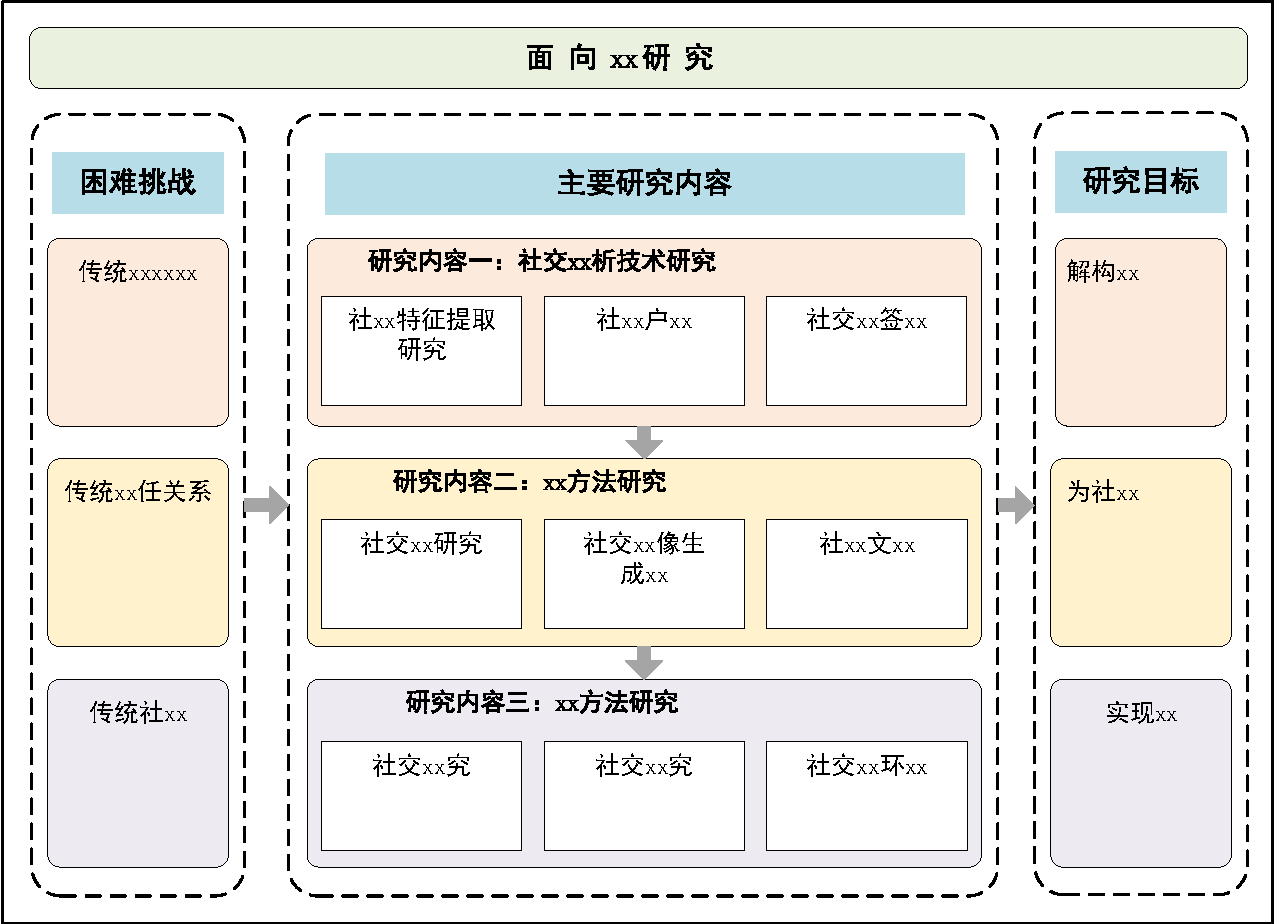
\includegraphics[scale=0.65]{Figures/ch1-research framework.pdf}
%	\caption{研究框架}
	\bicaption{研究框架}{Research framework}
	\label{fig:research framework}
\end{figure}

本文的研究工作主要包括:

\textbf{(1)研究一}

xxx


\textbf{(2)研究二}

xxx


\textbf{(3)研究三}

xxx

\subsection{研究创新}

基于上述研究内容,本文的创新如下:

\textbf{(1)创新一}

xxx

\textbf{(2)创新二}

xxx

\textbf{(3)创新三}

xxx

\section{文章结构}

本文共有六个章节,详细的阐述了xxxx的研究过程与结果。本文各章节具体内容安排如下:

第一章,绪论。本章首先介绍了xxx的背景与意义。其次,介绍了国内外关于xxx的研究现状。然后,详述了本文主要研究内容并归纳了本文的主要创新点。最后,叙述了本文的章节安排。

第二章,相关技术介绍。本章详述了本文涉及的相关技术,包括xxx、xx、xx、xx、xx。

第三章,研究一。本章首先xxx。其次,xxx。最后,xxx。

第四章,研究二。本章首先xxx。其次,xxx。最后,xxx。

第五章,研究三。本章首先xxx。其次,xxx。最后,xxx。

第六章,总结与展望。本章总结了本文全部研究内容,讨论了当前研究工作的不足,并指明了未来工作可能的研究方向。


